\documentclass[a4paper,landscape,oneside]{article}
\usepackage[pdftex,hidelinks]{hyperref}
\usepackage{fancyhdr}
\usepackage[
  headheight=35pt,
  headsep=15pt,
  footskip=20pt,
  includeheadfoot,
  hmargin=1cm,
  vmargin=0.75cm
]{geometry}
\usepackage{multirow}
\usepackage{tabularx}
\usepackage{tikz}

\pagestyle{fancy}
\tikzset{baseline=0,>=stealth}
\setlength{\parindent}{0pt}
\setlength{\tabcolsep}{10pt}
\renewcommand{\arraystretch}{1.5}

\newcounter{innernote}
\newcommand{\note}[1]{{\refstepcounter{innernote}\label{note:#1}\textsuperscript{\theinnernote}}}
\newcommand{\noteref}[1]{\textsuperscript{\ref{note:#1}}}

\title{Flatwater Kayaking}
\author{Jouke~Witteveen}

\makeatletter
\hypersetup{pdftitle=\@title,pdfauthor=\@author,pdfsubject={Technical Template: Physics}}
\lhead{}
\chead{
  \LARGE{\textbf{\@title}} \\[4pt]
  \large{Technical Template --- Physics}
}
\rhead{}
\lfoot{}
\cfoot{}
\rfoot{\small{\copyright{}~\the\year{} \@author}}
\makeatother


\begin{document}

\begin{tabularx}{\textwidth}{cp{9.7em}*{3}{|X}}
\multicolumn{2}{c}{}	& \multicolumn{3}{c}{
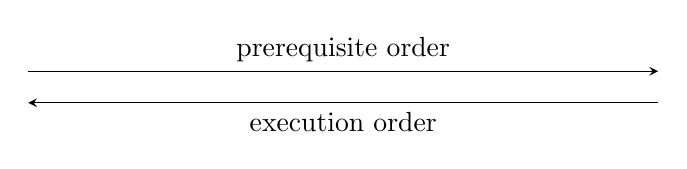
\begin{tikzpicture}
  \draw[->] (-4, 0.2) -- (4, 0.2) node[midway,above] {prerequisite order};
  \draw[<-] (-4, -0.2) -- (4, -0.2) node[midway,below] {execution order};
\end{tikzpicture}} \\[20pt]
\multicolumn{2}{c|}{}	& \multicolumn{1}{c|}{\emph{\textbf{Pull}}}	& \multicolumn{1}{c|}{\emph{\textbf{Entry}}}	& \multicolumn{1}{c}{\emph{\textbf{Set-up / Exit}}} \\
\cline{2-5}
\multirow{17}{*}{ % nrows = 3 + (lines - 3) / \arraystretch
\hspace{-20pt}
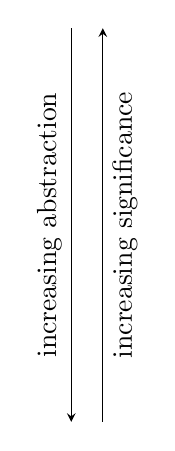
\begin{tikzpicture}
  \draw[<-] (-0.2, -2.5) -- (-0.2, 2.5) node[midway,sloped,above] {increasing abstraction};
  \draw[->] (0.2, -2.5) -- (0.2, 2.5) node[midway,sloped,below] {increasing significance};
\end{tikzpicture}
\hspace{0pt}}
& \emph{All applied forces must contribute to desirable acceleration.}\note{newton}
	& On average, the rearward directed force exerted on the water at the blade is matched by forward directed forces at the seat and footrest, as described by Newton's third law of motion.
	  This is the only source of forward acceleration of the boat.
	& In the reference frame of the boat, the paddle acts as a lever pushing against the resistance of the water.
	  The range of this lever is maximized by moving the fulcrum as far away from the load, the resistance of the water, as possible, hence as close to the top hand as possible, and by submersing the blade at maximum reach.
	& From some point in the stroke onward, the dominance of the backward directed component of the force exerted on the water at the blade starts to diminish.
	  The impact of unfavorable force components is limited through maintaining a high fulcrum and finishing the stroke with a distinct reduction of the applied force followed by a quick extraction of the blade from the water. \\
\cline{2-5}
& \emph{Hydrodynamic properties of the paddle blade and the hull of the boat must be utilized to maximize the yield from every stroke.}\note{lift}
	& The outward motion of the blade through the water generates a forward directed lift force on the blade.
	  The corresponding inward directed drag force is matched by the sideward resistance of the hull of the boat in the water, resulting in some sway.
	  Sideward acceleration of the center of mass is too restricted to prevent all sway.
	& When the blade enters the water sufficiently fast and at an appropriate angle, the downward motion of the blade through the water generates a forward directed lift force on the blade.
	  The corresponding upward directed drag force removes the downward directed component in the velocity of the blade.
	& There is not enough water over the submersed blade for the upward directed motion of the blade as it is extracted to generate a significant forward directed lift force.
	  The disturbance of the water surface, and with it the drag associated with the extraction of the blade, is minimized by extracting in an outward direction. \\
\cline{2-5}
& \emph{Acceleration of the center of mass must be decoupled from the velocity of the boat.}\note{velocity}
	& Forward acceleration of the center of mass varies during the stroke cycle.
	  While the center of mass is accelerated forward, not all of the associated force is required to overcome the drag force on the hull of the boat.
	  Acceleration of the center of mass forward relative to the boat reduces surge.
	& Heave as a result of the acceleration of the blade toward the water is negligible and not detrimental to the velocity.
	  Surge is suppressed by avoiding acceleration of the center of mass forward relative to the boat before a forward directed force is present on the blade.
	& In the absence of a force acting on the center of mass to match the drag force on the hull of the boat when no blade is interacting with the water, the velocity of the boat is maintained by acceleration of the center of mass backward relative to the boat.
\end{tabularx} \\[10pt]
\small{
\noteref{newton}
The available \emph{energy} is limited and exerting a force takes energy.
Therefore we want all applied forces to be beneficial to our velocity.

\noteref{lift}
As water moves past the boat, utilizing lift enables the exertion of a larger force with the same amount of \emph{work}.

\noteref{velocity}
Because drag increases roughly quadratically with the \emph{speed} of the boat, we want a maximum speed close to the average speed and the forces acting on the boat to be as constant as possible.
}
\vspace{\stretch{1}}

\small{
\emph{Velocity} is a directed physical quantity measuring the speed and direction with which the position of an object in motion changes.
The rate of change of the velocity of an object is its \emph{acceleration}.
As described by Newton's second law of motion, the \emph{force} acting on an object is directly proportional to its acceleration.
The coefficient of proportionality is the \emph{mass} of the object.
Mass is a conserved quantity, meaning it does not change over time in a closed system.
The point around which the distribution of the mass of an object is balanced is the object's \emph{center of mass}.
The overall force on an object can be thought of as acting on this point.
An object in motion through a fluid experiences a \emph{lift} force perpendicular to its motion.
Induced by the lift force, an object in motion through a fluid also experiences a \emph{drag} force that opposes the motion of the object.

\emph{Surge}, \emph{sway}, and \emph{heave} refer to variations in the velocity of a boat along its principal axes: forward--backward, side-to-side, and upward--downward, respectively.
}

\end{document}
